\subsection{Convolutional Neural Networks}
\label{sec:cnn-cnn}

Rule-based and closed-form solutions to image classification problems were the main stream techniques until the advent of deep CNNs. The AlexNet~\cite{AlexNet} in 2012's ImageNet contest suddenly improved the performance of image classifiers by a significant margin and profoundly changed the landscape of this research area.

CNNs are a class of neural networks based on convolutional layers which are modular sets of weights (convolutional filters) that operate on a small $m\times n$ patch of the input image at a time. The output of each filter is the dot-product between the weights and the pixels in the corresponding patch. Each filter is then \emph{convolved} with the input image, sliding across the entire image with a pre-determined stride and taking dot-products. It is important to note that the same set of weights for a given filter is used for the entire image otherwise the number of parameters for a CNN will explode and the network is impossible to train. The output of the operation is a new convolved image with size smaller or equal to the original image. A non-linear activation function is typically applied to each pixel of the convolved image.
Common to CNN architectures are non-covolutional down-sampling layers such as Max-pooling~\cite{MAXPOOL}.
Such layer takes non-overlapping patches of convolution outputs as input, and outputs the maximum value for each patch.
Typical CNNs are built with convolutional layers interleaved with pooling layers of different types. 

%The depth of the network is determined by the number of convolutions concatenated in the network.
%The sets of filters, the activations and the Max-pooling constitute the fundamental building block for CNNs.


\subsection{design and training of the q/g tagger}

The CNN architecture used in this study follows the example of Ref.~\cite{Komiske:2016rsd} and consists of three blocks of a convolutional layer with a
Rectified Linear Unit (ReLU) activation~\cite{RELU} and paired with a Max-pooling layer.
The last dense layer has 128 neurons with a ReLU activation taking in the flattened output from the convolutional blocks.
The output of the network is a softmax function~\cite{dlbook} of size two, 
predicting the probability for the quark jet and the gluon jet class, respectively. 
The convolutional layers consist of 128, 128 and 64 filters, with filter sizes of $5\times5$, $5\times5$ and $3\times3$, respectively.
The Max-pooling layers perform a $2\times2$ downsampling with a stride length of 2.
In order to prevent overfitting, dropout layer~\cite{Goodfellow-et-al-2016-Book} is applied to each convolution and the final fully connected layer with rate 0.3.
In addition, a L2 regularization~\cite{Goodfellow-et-al-2016-Book} with strength $10^{-8}$ is applied to all layers.  
A coarse scan of the various hyper-parameters was performed prior to settling on the architecture described above.
An illustration of the architecture used is shown in Figure~\ref{fig:networkarch}.

\begin{figure}[htpb]
\begin{center}
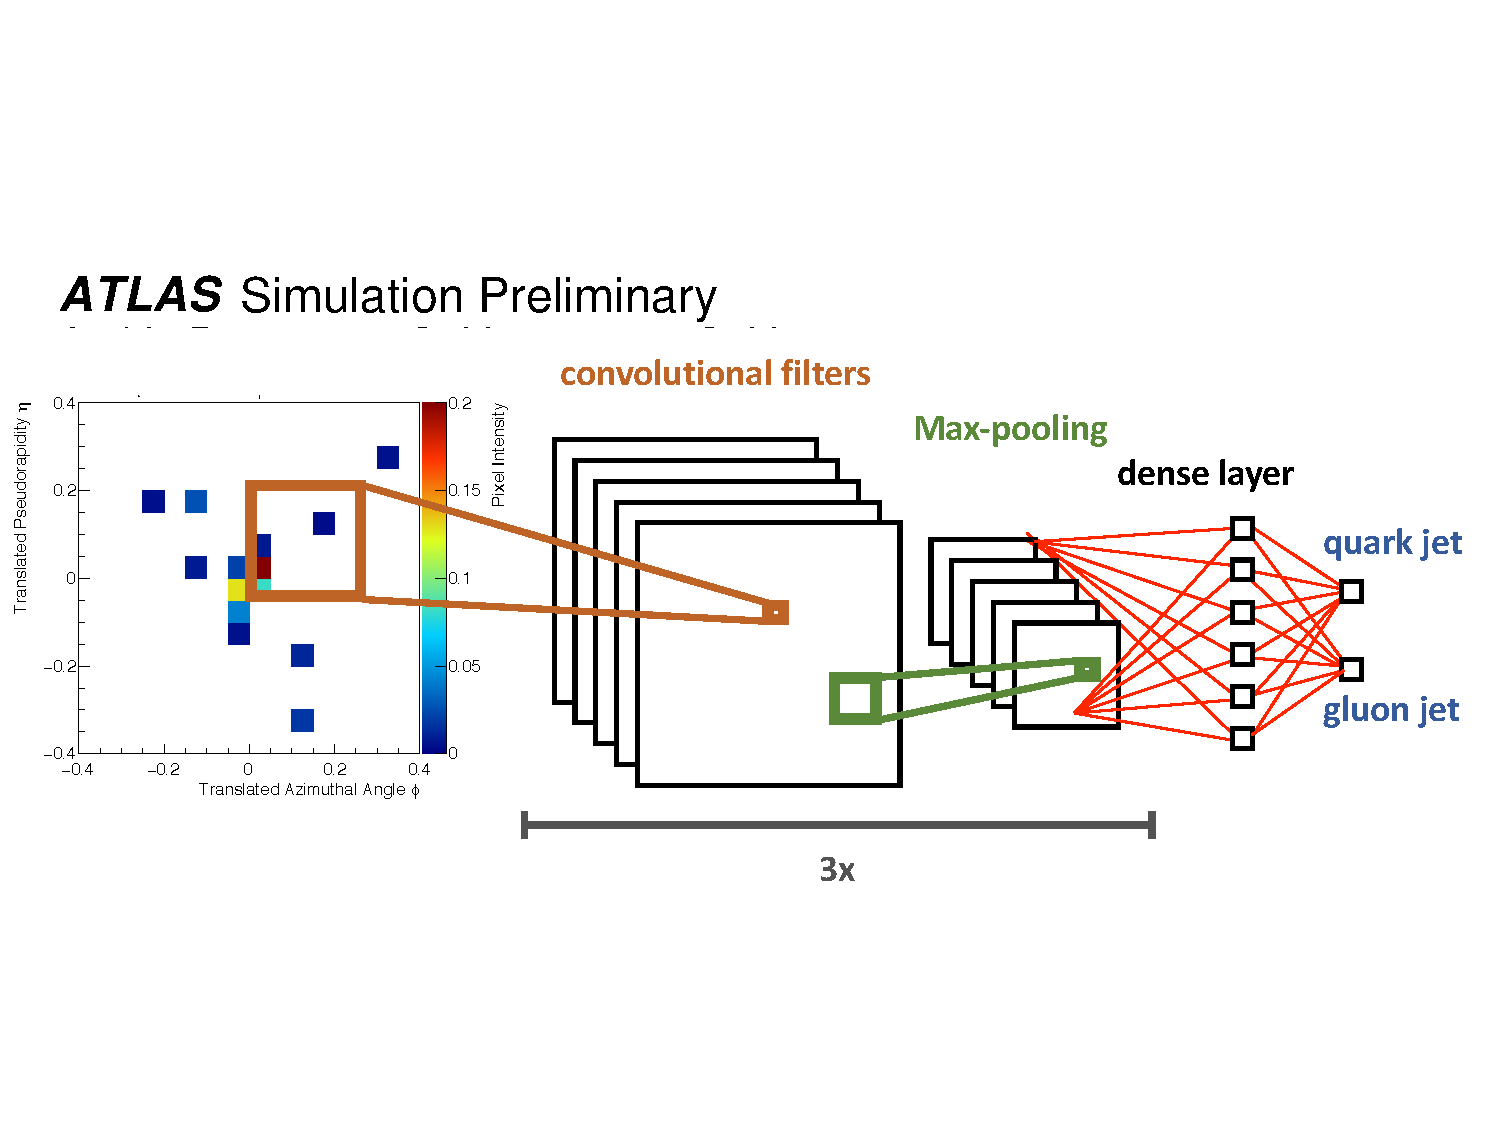
\includegraphics[width=0.8\textwidth]{figures/CNN/network.pdf}
\caption{Illustration of the deep convolutional neural network architecture.}
\label{fig:networkarch}
\end{center}
\end{figure}

Training is performed by minimizing the categorical crossentropy~\cite{Goodfellow-et-al-2016-Book}.
Minimization is performed with the Adam optimizer~\cite{DBLP:journals/corr/KingmaB14} 
as implemented in Keras~\cite{keras}
with a learning rate of 0.0001 over 50 iterations.
Training is performed using a single NVidia Tesla K80 GPU with 224000 jet images, while 56000 jet images are used for testing.
A typical training requires about 1 hour.
The network is retrained for each of the two $p_\text{T}$ ranges considered.
The output of the network corresponding to the quark jet class is used as a discriminant (\textit{CNN tagger}).
